\section{Experiments}
\label{sec:experiments}

% \begin{description}
% 	\item [RNN] 10, 25, 50, 75, and 100 gated recurrent units.
% 	\item [Training] 200 epochs.
% 	\item [Learning curves] cost functions, accuracies, and some metric for weights.
% 	\item[Activations] of GRUs for tunes.
% 	\item[Evaluation] on test set as a table.
% 	\item [Reconstructions] of test examples.
% \end{description}

The experiments were run for model 1, the normal RNN model using only original input and model 2, the extended RNN model using the previous prediction step output as input to the next step.

They are implemented in \Python with the \Theano and \Lasagne modules using mini-batch gradient descent with the Adam optimiser \cite{Kingma2014c} with a batch size of $10$ and learning rate of $0.005$.  

\subsection{Regularisation} % (fold)
\label{sub:regularization}

Dropout of $\SI{20}{\%}$ or $\SI{50}{\%}$ was applied right before the GRU layer in the input network. By dropping out notes along the melodies, a lossy noise and therefore a completion task is introduced to the models, so during training the next-step prediction will rely more on the previous GRU activations $\vec{h}\order{t-1}$ and the horizontal connections will be enhanced to make up for the missing input. The stronger horizontal connections will hopefully combine some more general musical rules and therefore reduce overfitting. 

An $L_2$-regularisation term is also added to the total cost during training to also reduce overfitting.

% subsection regularization (end)


\subsection{Evaluation}

The prediction accuracies for both pitches and durations are recorded for each epoch and their learning curves are shown in Figure~\ref{fig:learning_curves}.

\begin{figure*}
    \centering
    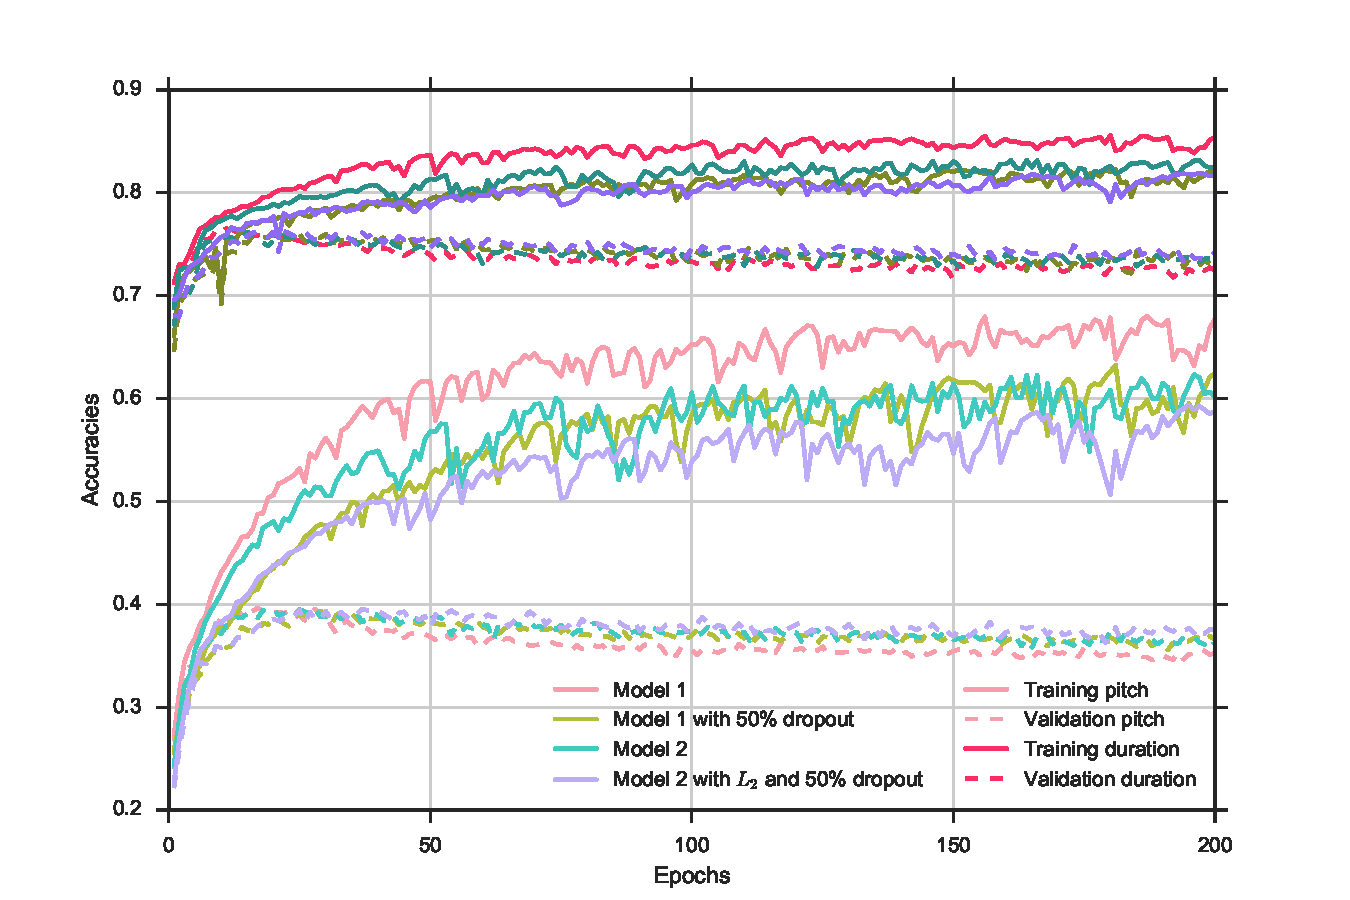
\includegraphics[width = 0.7\linewidth]{acc_learning_curves}
    \caption{Learning curves over next-step prediction accuracies for both model types with and without regularisation. The models are evaluated on both training (solid lines) and validation sets (dashed lines) for pitch (turquoise) and duration classes (orange).}
    \label{fig:learning_curves}
\end{figure*}

To investigate the connections in the GRU layer, the mean, Frobenius norm and positive-value fractions of horizontal and vertical weights are recorded and shown in Appendix~\ref{sec:gru_weights}, which are expected to show the trend in the overall magnitude and sign of the weights.

The two first models have been tested with and without dropout as well as with and without regularisation for $10$, $25$, $50$, $75$, and $100$ gated recurrent units, so scaling of performance can be investigated and the effect of the regularisation methods compared.
The third model was tested with and without $L_2$ regularisation.
The scaling of performance with the number of GRU are clearly seen, but not included here, so $100$ GRU are used as a standard and for these regularisation methods and model architectures can be compared for the test set in Table~\ref{tab:test_eval}.

\begin{table}
    \centering
    \caption{
        The test evaluation accuracies.
    }
    \label{tab:test_eval}
    % \setlength{\tabcolsep}{1em}
    \sisetup{
        table-number-alignment = center
    }
    \begin{tabular}{
            l@{}
            S[table-format = 1.0]
            S[table-format = 0.2]
            S[table-format = 1.0]
            S[table-format = 1.3]
            S[table-format = 1.3]
            S[table-format = 2.2]
            S[table-format = 2.2]
        }
        \toprule
        & {Model} 
        & {$p\idx{dropout}$}
        & {$\alpha_2$}
        % & {$L\idx{pitch}$}
        % & {$L\idx{duration}$}
        & {$A\idx{pitch}$(\%)}
        & {$A\idx{duration}$(\%)} \\
        \midrule
        \input{../data/eval_table}
        \bottomrule
    \end{tabular}
\end{table}

All models were trained for $200$ epochs, as they reach convergence after about $150$ epochs in the learning curves seen in Figure \ref{fig:learning_curves}.

\subsection{Reconstructions}

After training, the models were used to reconstruct several test melodies, and one was handpicked out of the unseen test set as an example for this report.
The first four bars of this melody is shown in Figure~\ref{fig:reconstructions} together with reconstructions using models~1 and~2.
In Appendix~\ref{sec:gru_activations}, the notes in the original melody are highlighted by colours corresponding to the GRU activations, so patterns, like scale and rhythmical motifs, leading to higher activation can be localised and the functionality of the GRU identified.

\begin{figure}
    \centering
    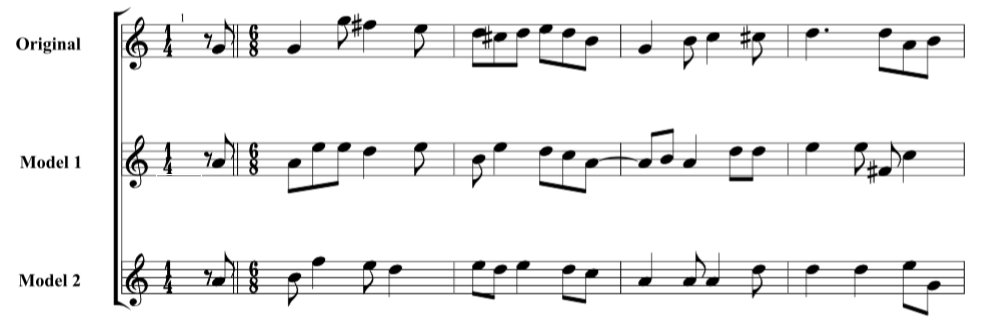
\includegraphics[width=\linewidth]{Reconstructions_cut}
    \caption{First 4 bars of notes in the melody, Fiddle Hill Jig, for original data and reconstructions produced by model 1 with dropout of 50\% and by model 2 with dropout of 50\% and $L_2$-regularisation.}
    \label{fig:reconstructions}
\end{figure}

To investigate the distribution of the pitch and duration classes, the frequencies of each class in the original data are represented in a histogram in Figure~\ref{fig:histogram}.

\begin{figure*}
    \centering
    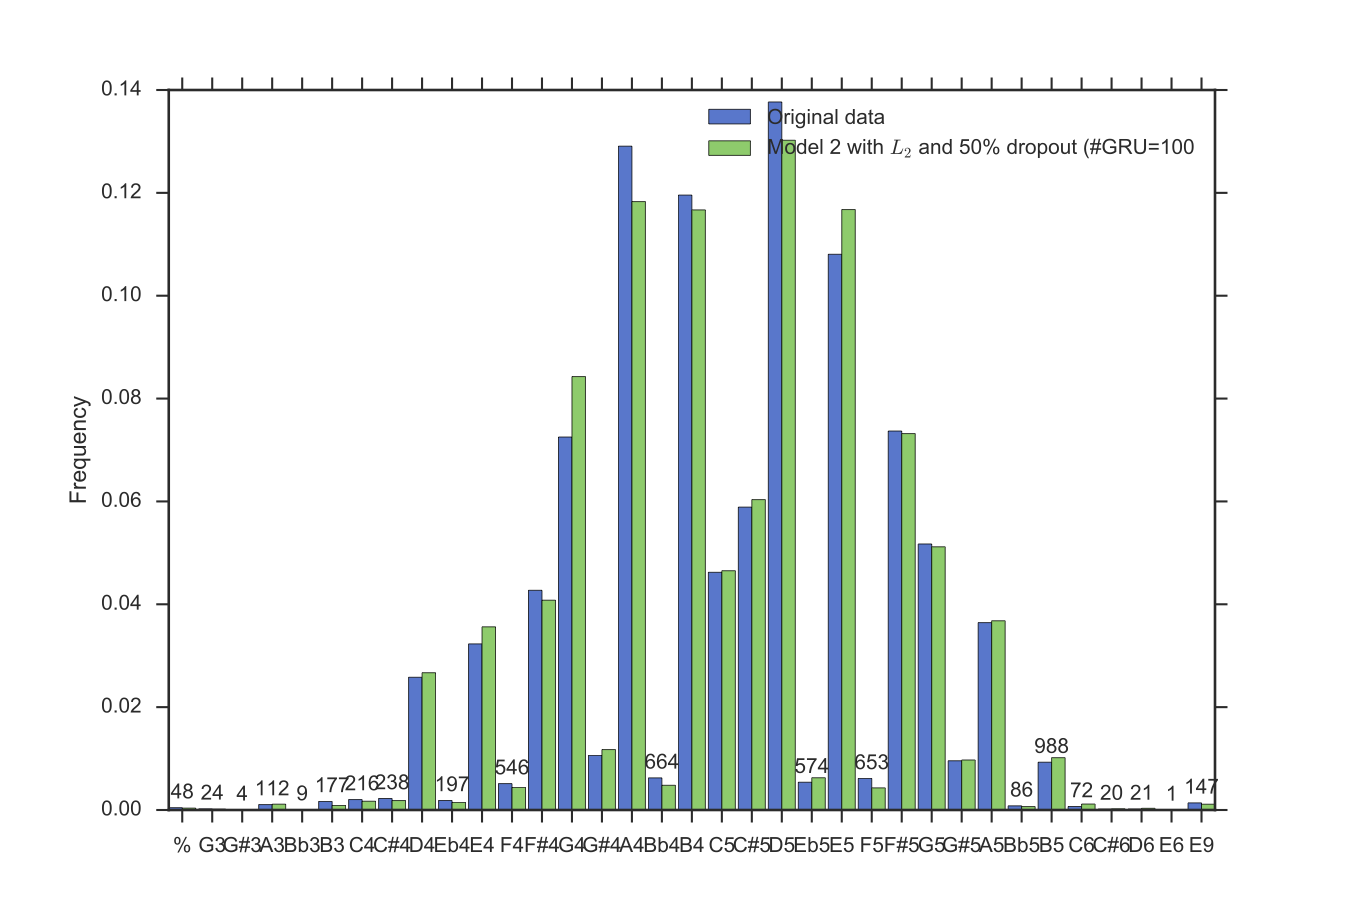
\includegraphics[width=.8\textwidth]{models_pitch_freq_barplot}
    \caption{Histograms showing statistical frequency of pitch classes in the (blue) original data and in the (green) reconstructions produced by model type 2 with dropout of 50\% and $L_2$-regularisation.}
    \label{fig:histogram}
\end{figure*}

All reconstructions can be converted to a musical notation, written to a MIDI file, played, written as a musical score and compared against the original melody.
